\documentclass[twoside]{article} % PREAMBLE

    \relax % Controls
        \newif\ifmarginprooflinks
        	\marginprooflinkstrue
        	% \marginprooflinksfalse

    \relax % Bibliography, etc
    	\usepackage[american]{babel}
    	\usepackage{csquotes}
    	\usepackage[backend=biber, style=authoryear]{biblatex}
    	\DeclareLanguageMapping{american}{american-apa}
    	% \usepackage[backend=biber,style=authoryear,hyperref=true]{biblatex}
    	\addbibresource{refs.bib}

    	\DeclareFieldFormat{citehyperref}{%
    	  \DeclareFieldAlias{bibhyperref}{noformat}% Avoid nested links
    	  \bibhyperref{#1}}

    	\DeclareFieldFormat{textcitehyperref}{%
    	  \DeclareFieldAlias{bibhyperref}{noformat}% Avoid nested links
    	  \bibhyperref{%
    	    #1%
    	    \ifbool{cbx:parens}
    	      {\bibcloseparen\global\boolfalse{cbx:parens}}
    	      {}}}

    	\savebibmacro{cite}
    	\savebibmacro{textcite}

    	\renewbibmacro*{cite}{%
    	  \printtext[citehyperref]{%
    	    \restorebibmacro{cite}%
    	    \usebibmacro{cite}}}

    	\renewbibmacro*{textcite}{%
    	  \ifboolexpr{
    	    ( not test {\iffieldundef{prenote}} and
    	      test {\ifnumequal{\value{citecount}}{1}} )
    	    or
    	    ( not test {\iffieldundef{postnote}} and
    	      test {\ifnumequal{\value{citecount}}{\value{citetotal}}} )
    	  }
    	    {\DeclareFieldAlias{textcitehyperref}{noformat}}
    	    {}%
    	  \printtext[textcitehyperref]{%
    	    \restorebibmacro{textcite}%
    	    \usebibmacro{textcite}}}

    	\DeclareCiteCommand{\brakcite}
    	  {\usebibmacro{prenote}}
    	  {\usebibmacro{citeindex}%
    	   \printtext[bibhyperref]{[\usebibmacro{cite}]}}
    	  {\multicitedelim}
    	  {\usebibmacro{postnote}}

    \relax % Standard Packages
        \usepackage[dvipsnames]{xcolor}
        % \usepackage[utf8]{inputenc}
        \usepackage{mathtools}
        \usepackage{amssymb}
    		\DeclareMathSymbol{\shortminus}{\mathbin}{AMSa}{"39}
        % \usepackage{parskip}
        % \usepackage{algorithm}
        \usepackage{bbm}
    	\usepackage{lmodern}
    	% \usepackage{times}
        \usepackage{faktor}
        % \usepackage{booktabs}
    	% \usepackage[margin=1in]{geometry}
        \usepackage{graphicx}
        \usepackage{scalerel}
        \usepackage{enumitem}
        \usepackage{nicefrac}\let\nf\nicefrac

        % \usepackage{color}
        %\usepackage{stmaryrd}
        \usepackage{hyperref} % Load before theorems...
            \hypersetup{colorlinks=true, linkcolor=blue!75!black, urlcolor=magenta, citecolor=green!50!black}

    \usepackage{tikz}
    	\usetikzlibrary{positioning,fit,calc, decorations, arrows, shapes, shapes.geometric}
    	\usetikzlibrary{cd}

    	%%%%%%%%%%%%
    	\tikzset{AmpRep/.style={ampersand replacement=\&}}
    	\tikzset{center base/.style={baseline={([yshift=-.8ex]current bounding box.center)}}}
    	\tikzset{paperfig/.style={center base,scale=0.9, every node/.style={transform shape}}}

    	% Node Stylings
    	\tikzset{dpadded/.style={rounded corners=2, inner sep=0.7em, draw, outer sep=0.3em, fill={black!50}, fill opacity=0.08, text opacity=1}}
    	\tikzset{dpad0/.style={outer sep=0.05em, inner sep=0.3em, draw=gray!75, rounded corners=4, fill=black!08, fill opacity=1, align=center}}
    	\tikzset{dpadinline/.style={outer sep=0.05em, inner sep=2.5pt, rounded corners=2.5pt, draw=gray!75, fill=black!08, fill opacity=1, align=center, font=\small}}

     	\tikzset{dpad/.style args={#1}{every matrix/.append style={nodes={dpadded, #1}}}}
    	\tikzset{light pad/.style={outer sep=0.2em, inner sep=0.5em, draw=gray!50}}

    	\tikzset{arr/.style={draw, ->, thick, shorten <=3pt, shorten >=3pt}}
    	\tikzset{arr0/.style={draw, ->, thick, shorten <=0pt, shorten >=0pt}}
    	\tikzset{arr1/.style={draw, ->, thick, shorten <=1pt, shorten >=1pt}}
    	\tikzset{arr2/.style={draw, ->, thick, shorten <=2pt, shorten >=2pt}}

    	\newcommand\cmergearr[5][]{
    		\draw[arr, #1, -] (#2) -- (#5) -- (#3);
    		\draw[arr, #1, shorten <=0] (#5) -- (#4);
    		}
    	\newcommand\mergearr[4][]{
    		\coordinate (center-#2#3#4) at (barycentric cs:#2=1,#3=1,#4=1.2);
    		\cmergearr[#1]{#2}{#3}{#4}{center-#2#3#4}
    		}
    	\newcommand\cunmergearr[5][]{
    		\draw[arr, #1, -, shorten >=0] (#2) -- (#5);
    		\draw[arr, #1, shorten <=0] (#5) -- (#3);
    		\draw[arr, #1, shorten <=0] (#5) -- (#4);
    		}
    	\newcommand\unmergearr[4][]{
    		\coordinate (center-#2#3#4) at (barycentric cs:#2=1.2,#3=1,#4=1);
    		\cunmergearr[#1]{#2}{#3}{#4}{center-#2#3#4}
    		}

    \usepackage{amsthm,thmtools} % Theorem Macros
    	\usepackage[noabbrev,nameinlink,capitalize]{cleveref}
        \theoremstyle{plain}
        \newtheorem{theorem}{Theorem}
    	\newtheorem{coro}{Corollary}[theorem]
        \newtheorem{prop}[theorem]{Proposition}
        \newtheorem{claim}{Claim}
        \newtheorem{remark}{Remark}
        \newtheorem{lemma}[theorem]{Lemma}
        \theoremstyle{definition}
        % \newtheorem{defn}{Definition}
        % \declaretheorem[name=Definition]{defn}
        \declaretheorem[name=Definition, qed=$\square$]{defn}
        \declaretheorem[name=Example, qed=$\triangle$]{example}

    	\crefname{defn}{Definition}{Definitions}
    	\crefname{prop}{Proposition}{Propositions}
        \crefname{issue}{Issue}{Issues}

    \relax %%%%%%%%% GENERAL MACROS %%%%%%%%
        \let\Horig\H
    	\let\H\relax
    	\DeclareMathOperator{\H}{\mathrm{H}} % Entropy
    	\DeclareMathOperator{\I}{\mathrm{I}} % Information
    	\DeclareMathOperator*{\Ex}{\mathbb{E}} % Expectation
    	\DeclareMathOperator*{\EX}{\scalebox{1.5}{$\mathbb{E}$}}

        \newcommand{\mat}[1]{\mathbf{#1}}
        \DeclarePairedDelimiterX{\infdivx}[2]{(}{)}{%
    		#1\;\delimsize\|\;#2%
    	}
    	\newcommand{\thickD}{I\mkern-8muD}
    	\newcommand{\kldiv}{\thickD\infdivx}
    	\newcommand{\tto}{\rightarrow\mathrel{\mspace{-15mu}}\rightarrow}

    	\newcommand{\datadist}[1]{\Pr\nolimits_{#1}}
    	% \newcommand{\datadist}[1]{p_\text{data}}

    	\makeatletter
    	\newcommand{\subalign}[1]{%
    	  \vcenter{%
    	    \Let@ \restore@math@cr \default@tag
    	    \baselineskip\fontdimen10 \scriptfont\tw@
    	    \advance\baselineskip\fontdimen12 \scriptfont\tw@
    	    \lineskip\thr@@\fontdimen8 \scriptfont\thr@@
    	    \lineskiplimit\lineskip
    	    \ialign{\hfil$\m@th\scriptstyle##$&$\m@th\scriptstyle{}##$\hfil\crcr
    	      #1\crcr
    	    }%
    	  }%
    	}
    	\makeatother
    	\newcommand\numberthis{\addtocounter{equation}{1}\tag{\theequation}}

    \relax %%%%%%%%%   PDG  MACROS   %%%%%%%%
    	\newcommand{\ssub}[1]{_{\!_{#1}\!}}
    	% \newcommand{\bp}[1][L]{\mat{p}_{\!_{#1}\!}}
    	% \newcommand{\bP}[1][L]{\mat{P}_{\!_{#1}\!}}
    	\newcommand{\bp}[1][L]{\mat{p}\ssub{#1}}
    	\newcommand{\bP}[1][L]{\mat{P}\ssub{#1}}
    	\newcommand{\V}{\mathcal V}
    	\newcommand{\N}{\mathcal N}
    	\newcommand{\Ed}{\mathcal E}

        \newcommand{\balpha}{\boldsymbol\alpha}
        \newcommand{\bbeta}{\boldsymbol\beta}

    	\DeclareMathAlphabet{\mathdcal}{U}{dutchcal}{m}{n}
    	\DeclareMathAlphabet{\mathbdcal}{U}{dutchcal}{b}{n}
    	\newcommand{\dg}[1]{\mathbdcal{#1}}
    	\newcommand{\PDGof}[1]{{\dg M}_{#1}}
    	\newcommand{\UPDGof}[1]{{\dg N}_{#1}}
    	\newcommand\VFE{\mathit{V\mkern-4mu F\mkern-4.5mu E}}

    	\newcommand\Inc{\mathit{Inc}}
    	\newcommand{\IDef}[1]{\mathit{IDef}_{\!#1}}
    	% \newcommand{\ed}[3]{%
    	% 	\mathchoice%
    	% 	{#2\overset{\smash{\mskip-5mu\raisebox{-3pt}{${#1}$}}}{\xrightarrow{\hphantom{\scriptstyle {#1}}}} #3} %display style
    	% 	{#2\overset{\smash{\mskip-5mu\raisebox{-3pt}{$\scriptstyle {#1}$}}}{\xrightarrow{\hphantom{\scriptstyle {#1}}}} #3}% text style
    	% 	{#2\overset{\smash{\mskip-5mu\raisebox{-3pt}{$\scriptscriptstyle {#1}$}}}{\xrightarrow{\hphantom{\scriptscriptstyle {#1}}}} #3} %script style
    	% 	{#2\overset{\smash{\mskip-5mu\raisebox{-3pt}{$\scriptscriptstyle {#1}$}}}{\xrightarrow{\hphantom{\scriptscriptstyle {#1}}}} #3}} %scriptscriptstyle
    	\newcommand{\ed}[3]{#2%
    	  \overset{\smash{\mskip-5mu\raisebox{-1pt}{$\scriptscriptstyle
    	        #1$}}}{\rightarrow} #3}

        \newcommand{\nhphantom}[2]{\sbox0{\kern-2%
    		\nulldelimiterspace$\left.\delimsize#1\vphantom{#2}\right.$}\hspace{-.97\wd0}}
    		% \nulldelimiterspace$\left.\delimsize#1%
    		% \vrule depth\dp#2 height \ht#2 width0pt\right.$}\hspace{-.97\wd0}}
    	\makeatletter
    	\newsavebox{\abcmycontentbox}
    	\newcommand\DeclareDoubleDelim[5]{
    	    \DeclarePairedDelimiterXPP{#1}[1]%
    			{% box must be saved in this pre code
    				\sbox{\abcmycontentbox}{\ensuremath{##1}}%
    			}{#2}{#5}{}%
    		    %%% Correct spacing, but doesn't work with externalize.
    			% {\nhphantom{#3}{##1}\hspace{1.2pt}\delimsize#3\mathopen{}##1\mathclose{}\delimsize#4\hspace{1.2pt}\nhphantom{#4}{##1}}
    			%%% Fast, but wrong spacing.
    			% {\nhphantom{#3}{~}\hspace{1.2pt}\delimsize#3\mathopen{}##1\mathclose{}\delimsize#4\hspace{1.2pt}\nhphantom{#4}{~}}
    			%%% with savebox.
    		    {%
    				\nhphantom{#3}{\usebox\abcmycontentbox}%
    				\hspace{1.2pt} \delimsize#3%
    				\mathopen{}\usebox{\abcmycontentbox}\mathclose{}%
    				\delimsize#4\hspace{1.2pt}%
    				\nhphantom{#4}{\usebox\abcmycontentbox}%
    			}%
    	}
    	\makeatother
    	\DeclareDoubleDelim
    		\SD\{\{\}\}
    	\DeclareDoubleDelim
    		\bbr[[]]
    	% \DeclareDoubleDelim
    	% 	\aar\langle\langle\rangle\rangle
    	\makeatletter
    	\newsavebox{\aar@content}
    	\newcommand\aar{\@ifstar\aar@one@star\aar@plain}
    	\newcommand\aar@one@star{\@ifstar\aar@resize{\aar@plain*}}
    	\newcommand\aar@resize[1]{\sbox{\aar@content}{#1}\scaleleftright[3.8ex]
    		{\Biggl\langle\!\!\!\!\Biggl\langle}{\usebox{\aar@content}}
    		{\Biggr\rangle\!\!\!\!\Biggr\rangle}}
    	\DeclareDoubleDelim
    		\aar@plain\langle\langle\rangle\rangle
    	\makeatother


    	% \DeclarePairedDelimiterX{\aar}[1]{\langle}{\rangle}
    	% 	{\nhphantom{\langle}{#1}\hspace{1.2pt}\delimsize\langle\mathopen{}#1\mathclose{}\delimsize\rangle\hspace{1.2pt}\nhphantom{\rangle}{#1}}

    \relax %%%%% restatables and links
    	% \usepackage{xstring} % for expandarg
    	\usepackage{xpatch}
    	\makeatletter
    	\xpatchcmd{\thmt@restatable}% Edit \thmt@restatable
    	   {\csname #2\@xa\endcsname\ifx\@nx#1\@nx\else[{#1}]\fi}% Replace this code
    	   % {\ifthmt@thisistheone\csname #2\@xa\endcsname\typeout{oiii[#1;#2\@xa;#3;\csname thmt@stored@#3\endcsname]}\ifx\@nx#1\@nx\else[#1]\fi\else\csname #2\@xa\endcsname\fi}% with this code
    	   {\ifthmt@thisistheone\csname #2\@xa\endcsname\ifx\@nx#1\@nx\else[{#1}]\fi
    	   \else\fi}
    	   {}{\typeout{FIRST PATCH TO THM RESTATE FAILED}} % execute on success/failure
    	\xpatchcmd{\thmt@restatable}% A second edit to \thmt@restatable
    	   {\csname end#2\endcsname}
    	   {\ifthmt@thisistheone\csname end#2\endcsname\else\fi}
    	   {}{\typeout{FAILED SECOND THMT RESTATE PATCH}}

    	% \def\onlyaftercolon#1:#2{#2}
    	\newcommand{\recall}[1]{\medskip\par\noindent{\bf \Cref{thmt@@#1}.} \begingroup\em \noindent
    	   \expandafter\csname#1\endcsname* \endgroup\par\smallskip}

       	\setlength\marginparwidth{1.55cm}
    	\newenvironment{linked}[3][]{%
    		\def\linkedproof{#3}%
    		\def\linkedtype{#2}%
    		% \reversemarginpar
    		% \marginpar{%
    		% \vspace{1.1em}
    		% % \hspace{2em}
    		% 	% \raggedleft
    		% 	\raggedright
    		% 	\hyperref[proof:\linkedproof]{%
    		% 	\color{blue!50!white}
    		% 	\scaleleftright{$\Big[$}{\,{\small\raggedleft\tt\begin{tabular}{@{}c@{}} proof of \\\linkedtype~\ref*{\linkedtype:\linkedproof}\end{tabular}}\,}{$\Big]$}}
    		% 	}%
            % \restatable[#1]{#2}{#2:#3}\label{#2:#3}%
    		\ifmarginprooflinks
    		\marginpar{%
    			% \vspace{-3em}% %% for bottom
    			\vspace{1.5em}
    			\centering%
    			\hyperref[proof:\linkedproof]{%
                % \hyperref[proof:#3]{
    			\color{blue!30!white}%
    			\scaleleftright{$\Big[$}{\,\mbox{\footnotesize\centering\tt\begin{tabular}{@{}c@{}}
    				% proof of \\\,\linkedtype~\ref*{\linkedtype:\linkedproof}
    				link to\\[-0.15em]
    				proof
    			\end{tabular}}\,}{$\Big]$}}~
    			}%
    		\fi
            \restatable[#1]{#2}{#2:#3}\label{#2:#3}%
            }%
    		{\endrestatable%
    		}
    	\makeatother
    		\newcounter{proofcntr}
    		\newenvironment{lproof}{\begin{proof}\refstepcounter{proofcntr}}{\end{proof}}

    		\usepackage{cancel}
    		\newcommand{\Cancel}[2][black]{{\color{#1}\cancel{\color{black}#2}}}

    		\usepackage{tcolorbox}
    		\tcbuselibrary{most}
    		\tcolorboxenvironment{lproof}{
    			% fonttitle=\bfseries,
    			% top=0.5em,
    			enhanced,
    			parbox=false,
    			boxrule=0pt,
    			frame hidden,
    			borderline west={4pt}{0pt}{blue!20!black!40!white},
    			% coltext={blue!20!black!60!white},
    			colback={blue!20!black!05!white},
    			sharp corners,
    			breakable,
    			% bottomsep at break=4cm,
    			% enlarge bottom at break by=-4cm,
    			% topsep at break=3cm,
    			% enlarge top at break by=-3cm
    		}
    		% \usepackage[framemethod=TikZ]{mdframed}
    		% \surroundwithmdframed[ % lproof
    		% 	   topline=false,
    		% 	   linewidth=3pt,
    		% 	   linecolor=gray!20!white,
    		% 	   rightline=false,
    		% 	   bottomline=false,
    		% 	   leftmargin=0pt,
    		% 	   % innerleftmargin=5pt,
    		% 	   skipabove=\medskipamount,
    		% 	   skipbelow=\medskipamount
    		% 	]{lproof}
    	%oli16: The extra space was because there was extra space in the paragraph, not
    	%because this length was too big. By breaking arrays, everything will be better.
    	\newcommand{\begthm}[3][]{\begin{#2}[{name=#1},restate=#3,label=#3]}

    \relax %TODOs and footnotes
        \newcommand{\TODO}[1][INCOMPLETE]{{\centering\Large\color{red}$\langle$~\texttt{#1}~$\rangle$\par}}
        \newcommand{\dfootnote}[1]{%
            \let\oldthefootnote=\thefootnote%
            % \addtocounter{footnote}{-1}%
    		\setcounter{footnote}{999}
            \renewcommand{\thefootnote}{\textdagger}%
            \footnote{#1}%
            \let\thefootnote=\oldthefootnote%
        }
    	\newcommand{\dfootnotemark}{
    		\footnotemark[999]
    	}

% \twocolumn
\setlength\parskip{1ex}
% \usepackage[margin=1.2in]{geometry}

% \usepackage{arabtex}


\begin{document}
    Even though they seem to enable some very interesting modeling behavior from PDGs, the weight parameters $\balpha$ and $\bbeta$ suffer from some issues.

    \begin{enumerate}[label={Issue \arabic*.}, ref={\arabic*}]
        \item  We have used the word ``confidence'' for both $\alpha$ and $\beta$, despite the fact that they effectively have different ranges and units.
            \label[issue]{issue:conflictconfidence}
        \item We would like the notion of a PDG not to be too wedded to its semantics. As nice as the semantics are, the syntactic specification is even more natural, and we do not want to preclude the possibility of further semantic interpretations simplly because of the way we have articulated the confidence parameters $\balpha$ and $\bbeta$.
            \label[issue]{issue:multisemantics}
    \end{enumerate}


    % Perhaps the best way to address \cref{issue:multisemantics} is by considering alternate semantics.
    %TODO
    % \Cref{issue:conflictconfidence}
    %
    In this document, we consider two approaches to address these issues and make $\balpha$ and $\bbeta$ more interpretable, corresponding to \cref{sec:trust-dominance,sec:sticking-to-confidence}. We then combine the approaches in \cref{sec:analysis}

    \section{Sticking with ``Confidences''} 
        \label{sec:sticking-to-confidence}
        
    % Let {\RL{b}}.
    One alternative to specifying $\beta \in [0, \infty]$ is to 

    to specify $\tilde\beta \in [0,1]$, plus a cofficient $\gamma'$, and define
    $
        \beta := - \log ({1-\tilde\beta})
    $
    so that
    \begin{align*}
        \bbr{\dg M}_{\gamma,\gamma'}
            &= \gamma' \Inc_{\dg M}(\mu) + \gamma \IDef{\dg M}(\mu) \\
            &= \Ex_{\mu} \left[
                \sum_{\ed LXY} \gamma' \log \frac1{1-\tilde\beta}\cdot\log \frac{\mu(Y|X)}{\bp(Y|X)}  + \gamma \alpha \log \mu(Y|X)
                \right]
    \end{align*}



    \section{Trust and Dominance}\label{sec:trust-dominance}
    A particularly simple  solution to \cref{issue:conflictconfidence} is to slightly alter the names and interpretations of the parameters to clarify their differences and their roles in the model.
    Indeed, even if we reparameterize, 
    if we are to retain the PDG semantics the way that they currently work.

    I propose calling $\bbeta$ ``trust'', and $\balpha$ ``dominance''.




    \subsection{Trust}
    We measure trust in $\bbeta$ disutility per error.
    Each unit of discrepency a highly trusted information and reality is painful (the pain of betrayed trust).
    % We submit that this is a reasonable way to measure trust:
    Furthermore, errors in highly trusted information are very costly, while untrusted sources have relatively little potential for betrayal.


    In some ways, this is a new approach, but it is closely related to previous formuluations of $\bbeta$, which we now detail.
    The hope is that this presentation skirts some of the others' issues; we now enumerate some of those other approaches.
    \smallskip
    \begin{enumerate}
        \item $\bbeta$ \textbf{as Value of Information.} You are willing to pay more (in dollars per bit) for more-trusted information than for less-trusted information.

        Some issues:
        \begin{itemize}
                % [nosep]
            \item How much you'd be willing to pay depends not only on the currency you're paying in, but also on the context. Why do you need it? Are there other sellers?
            %
              None of this is important; in this setting, ``value'' is to be interpreted vaguely.
              By analogy, consider expected utility. When asked for your preference between two bets, you're not allowed to say ``it depends on this other variable $Z$''; you must instead give your preference and do your best to account for $Z$.

            Still, this interaction with pragmatics could be problematic for us later on. If we later use PDGs to model an agent that also has a clear use for certain information, we do not want the ``value of information'' interpretation to torque the value of $\beta$. Instead, we would like $\beta$ to be specified blindly to this context.

            The hope is that ``pain of betrayal'' is better-suited even in this context.
            To start, misinformation even about seemingly unimportant variables, can reverberate, subtly impacting important information as well (the existence of side-channel attacks is proof of this).
            Futhermore, if one gets a new instrumental goal or arrives in a new context, previously unimportant information may suddenly become important.
            For these reasons, it makes sense that trust, as measured by disutility of betrayal, would be substantially more robust to this kind of consideration.

            \item Utility is subjective. This subjectivity is also a feature of our presentation `trust', but came up as a potential issue in our last meeting.
            I don't think it's problematic. See \cref{disutility:subjective}.
        \end{itemize}

        \item $\bbeta$ \textbf{as Confidence.}
        We have been calling this same value $\beta$ ``confidence'', often a synonym for ``trust''.
        % For the same reasons as above,
        High-confidence beliefs, just like highly trusted ones, should result in more internal conflict per violation, while low-confidence beliefs, like untrusted ones, should result in less internal conflict per violation.

        The major issue is that  ``confidence'' is often reserved for probabilities in $[0,1]$, which is particularly problematic if $\alpha$, which is more often thought of in this way, is also called a ``confidence'' of sorts.

        \item $\bbeta$ \textbf{as Usage.}
        The defense of the semantics in the Inconsistency-as-loss paper also uses frequency of use as an intermediate.
        \begin{quote}\it
            ``But if one uses edges in proportion to the confidence one has in
            them, then $\mu$'s violations of high-confidence cpds are compounded,
            and hence more costly.''
        \end{quote}
        I view this as a weak illustration that $\beta$ should combine additively be measured on a ratio scale: zero is special because it corresponds to no use, but in general $\beta$ can be unbounded.
        However, viewing $\beta$ as ``usage'' is totally useless as a way of \emph{choosing} the parameter $\beta$. Usage, even more so than value-of-information, is influenced by irrelevant factors.

        As such, the phrase ``if one uses edges in proportion to the confidence the modeler has in them'' does a lot of work. Mostly this approach rests on the notion of confidence.
    \end{enumerate}
    \smallskip

    \noindent In each case, $\beta_L$ can be measured in units of
     % $\frac{\text{value}}{\text{information}}$.
    value per information.

    Some additional thoughts on the word ``trust'':
    \begin{itemize}
        \item It is a close synonym of ``confidence'', which was the original presentation.

        \item It also has a standard meaning in terms of capital: a trust is in some sense a financial asset, often in the form of a portfolio of investments optimized for stability. Its magnitude can be measured in dollars.
        Furthermore, an investment portfolio in some sense reflects probabilistic beliefs (they are bets about what is likely to go up and down in value), and because the point is stability, the capital is concentrated in beliefs one has high confidence in.

        \item Interpreting $\beta$ as ``pain of betrayal arising from inaccuracy'' gives us an intuitive meaning if it is negative: the vindication of seeing information you actively \emph{distrust} proven wrong.
        \item I think the notion of trust is actually much more continuous than its representation in the security literature would have one believe. I think that modeling trust and its dynamics is extremely important, and I have strong intuition that $\beta$ captures useful features of it.

        That said, it remains to be seen whether PDGs can produce interesting results for analyzing trust, and how it will play with a multi-agent picture of PDGs, when we get to that.
    \end{itemize}



    \subsubsection{On Subjectivenss of Utility: Is it a Problem?}
    \label{disutility:subjective}

    The whole point of (expected) utility is that you can use it to numerically compare outcomes in goodness. It comes with the

    It is true that utility is not comparable across different people, but really the point is that the pain of betrayal of one belief versus another can be traded off.
    The actual values of the numbers can be different and you can have an equivalent model\footnote{for instance, one can always double $\bbeta$ and $\gamma$ to double the scoring function, resulting in the same optima and qualitative features}.


    \subsubsection{Dynamics}
    One option is to have
    \[
        \dot\bbeta = -\eta \nabla_{\bbeta} \aar{\dg M}
    \]


    \[
        \dot\beta\ssub L = -\eta \frac{1}{{\beta\ssub L}^2} \frac{\partial \aar{\dg M}}{\partial \beta\ssub L}
    \]


    \textbf{Hebbian Dynamics.}
    The rate of change of the connection $w_{i,j}$ between neurons $i$ and $j$ changes in proportion to $w_{i,j} \cdot C_{i,j}$ where $C_{i,j}$ is the correlation between $i$ and $j$.
    \[
        \frac{\mathrm d \bbeta}{\mathrm d t}
             =
    \]


    \subsection{Dominance}
    % Dominance, on the other hand, is unitless; it is specified relative to
    \begin{center}
        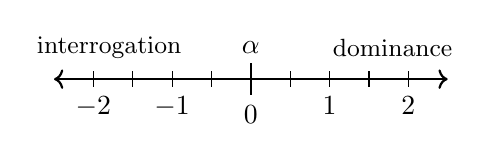
\begin{tikzpicture}
            \draw[thick, <->] (-2.5,0) -- (2.5, 0);
            \foreach \x in {-2.0, -1.5, ..., 2.0} {
                \draw[thin] (\x, 0.1) -- (\x,-0.1);
            }
            \foreach \x in {-2, -1, 1, 2} {
                \draw[thin] (\x, 0.1) -- (\x,-0.1) node[below]{$\x$};
            }
            \draw[thick] (0,0.2) -- (0,-0.2) node[below] {$0$};
            \node at  ( 0 , 0.4) {$\alpha$};
            \node[font=\small] at ( 1.8, 0.4) {dominance};
            \node[font=\small] at (-1.8, 0.4) {interrogation};

        \end{tikzpicture}
    \end{center}
    Dominance, on the other hand, is relative to

    \TODO
    Interrogative strength.




    \section{Comparison and Analysis} \label{sec:analysis}
    I find the former to be the cleaner approach. It leaves the interpretation more closely related to its usage in the semantics, which, despite flying in the face of \cref{issue:multisemantics}, means that:

    \begin{itemize}
        \item The formula we write for the scoring function is simpler and more natural.
            We don't need to
        \item we don't require the extra parameter $\gamma'$, and

    \end{itemize}



    %%%%%%%%%%%%%%%%%%%%%%%%%%%%%%%%%%%%%%%%%%%%%%%%%%%%%%%%%%%%%%%%%%%%%
\clearpage
    \section*{Playing With Flow and Chemical Equilibrium}
    Can we think of $\beta$ as a rate constant?

    \begin{defn}
        A distribution of capital is a function $\$ : \sum \V \to \mathbb R^+$.
        For instance, if a PDG contains the two variables $A$ and $B$, with $\V(A) = \{a_1, a_2\}$ and $\V(B) = \{b_1, b_2, b_3\}$, then $\$$ consists of the five numbers
        \[
            \$(A\!=\!a_1),\quad
            \$(A\!=\!a_2),\quad
            \$(B\!=\!b_1),\quad
            \$(B\!=\!b_2),\quad\text{and}\quad
            \$(B\!=\!b_3).
        \]
    \end{defn}


    % We can think of it as a concentration.
    We can then define a flow of of capital by

    \begin{align*}
        \frac{\mathrm d \$(x) }{\mathrm dt} &=
            \overbrace{%
                \sum_{\ed LZX} \sum_{z \in \V(Z)} \bp(x\,|\,z) \$(Z=z)-\$(X=x)
            }^{\text{flow in from variables $Z$}} \\
            &\qquad -
                \underbrace{%
                \sum_{\ed LXY} \sum_{y \in \V(Z)} \bp(y\,|\,x) \$(X=x)-\$(Y=y)
                }_{\text{flow out to variables $Y$}}
            \\
            &= \sum_{\ed LZX} \sum_z (\bp(x\,|\,z) \$(z)-\$(x))
                -\sum_{\ed LXY} \Big(\$(x)\sum_{y} \bp(y\,|\,x) - \$(Y) \Big) \\
            &= \sum_{\ed LZX} \sum_z (\bp(x\,|\,z) \$(z)-\$(x))
                -\sum_{\ed LXY} \Big(\$(x) - \$(Y) \Big)
            .
    \end{align*}


    The hope is that a joint distribution $\mu : \Delta \V(\dg M)$ can be viewed as an ``echo'' of the the flow through the system.


    \begin{example}

    \end{example}


\end{document}
